\section{Auswertung}
\label{sec:Auswertung}
In Tabelle \ref{tab:messung1} sind die Gemessenden Wertepaare für die Messreihe $p<1\si{\bar}$
angegeben. In Abbildung \ref{fig:fit1} wird der Dampfdruck logarithmisch in Abhängigkeit
zum Kehrwert der Temperatur aufgetragen. Der dazugehörige Fit hat nach Gleichung
\eqref{eqn:loesung_dgl} die Form
\begin{equation}
  \ln p=-\frac{A}{RT}+B
\end{equation}
mit den Fitparametern
\begin{align*}
  A=&\SI{3.94(6)e4}{\frac{\joule}{\mol}}\\
  B=&\SI{1.96(2)e1}{}\;\;.
\end{align*}
Damit ist die gemittelte Verdampfungswärme $L=\SI{3.94(6)e4}{\frac{\joule}{\mol}}$.
Die äußere Verdampfungswärme $L_a$ ist die benötigte Energie um das Volumen eines
Mols einer Flüssigleit auf das Volumen des Gases zu vergrößern. Daher ergibt sich
mit dem Wert $T=373\si{\kelvin}$ die äußere Verdampfungswärme
\begin{equation}
  L_a=pV=RT=\SI{3102.540674(6)}{\frac{\joule}{\mol}}\;\;.
\end{equation}
Die innere Verdampfungswärme ist damit
\begin{equation}
  L_i=L-L_a=\SI{3.63(6)e4}{\frac{\joule}{\mol}}\;\;.
\end{equation}
um die innere Verdampfungswärme $L_i$ für ein Molekül zu erhalten, muss das Ergebnis
durch ein $\si{\mol}$ geteilt werden. So das für ein Molekül die innere Verdampfungswärme
in Electronenvolt $L_i=\SI{0.376(6)}{\electronvolt}$ ist.
\begin{table}
  \centering
  \begin{tabular}{c c c c}
    \toprule
    Temperatur & Druck \\
    $T$ in $\si{\kelvin}$ & $p$ in $ 10^2\si{\pascal}$ &  & \\
    \midrule
    328.15  &   183  &    &  \\
    329.65  &   192  &    &  \\
    331.15  &   201  &    &  \\
    332.65  &   218  &    &  \\
    334.15  &   233  &    &  \\
    338.15  &   255  &    &  \\
    341.15  &   283  &    &  \\
    344.15  &   323  &    &  \\
    347.15  &   369  &    &  \\
    350.15  &   424  &    &  \\
    353.15  &   476  &    &  \\
    356.15  &   548  &    &  \\
    359.15  &   608  &    &  \\
    362.15  &   681  &    &  \\
    365.15  &   766  &    &  \\
    368.15  &   845  &    &  \\
    371.15  &   956  &    &  \\
   1374.15  &  1047  &    &  \\
    \bottomrule
  \end{tabular}
  \caption{Dampfdruck und Temperatur mit einer Messungenauigkeit von
  $\Delta T=0.1\si{\kelvin}$ und $\Delta p=100 \si{\pascal}$.}
  \label{tab:messung1}
\end{table}
\begin{figure}
  \centering
  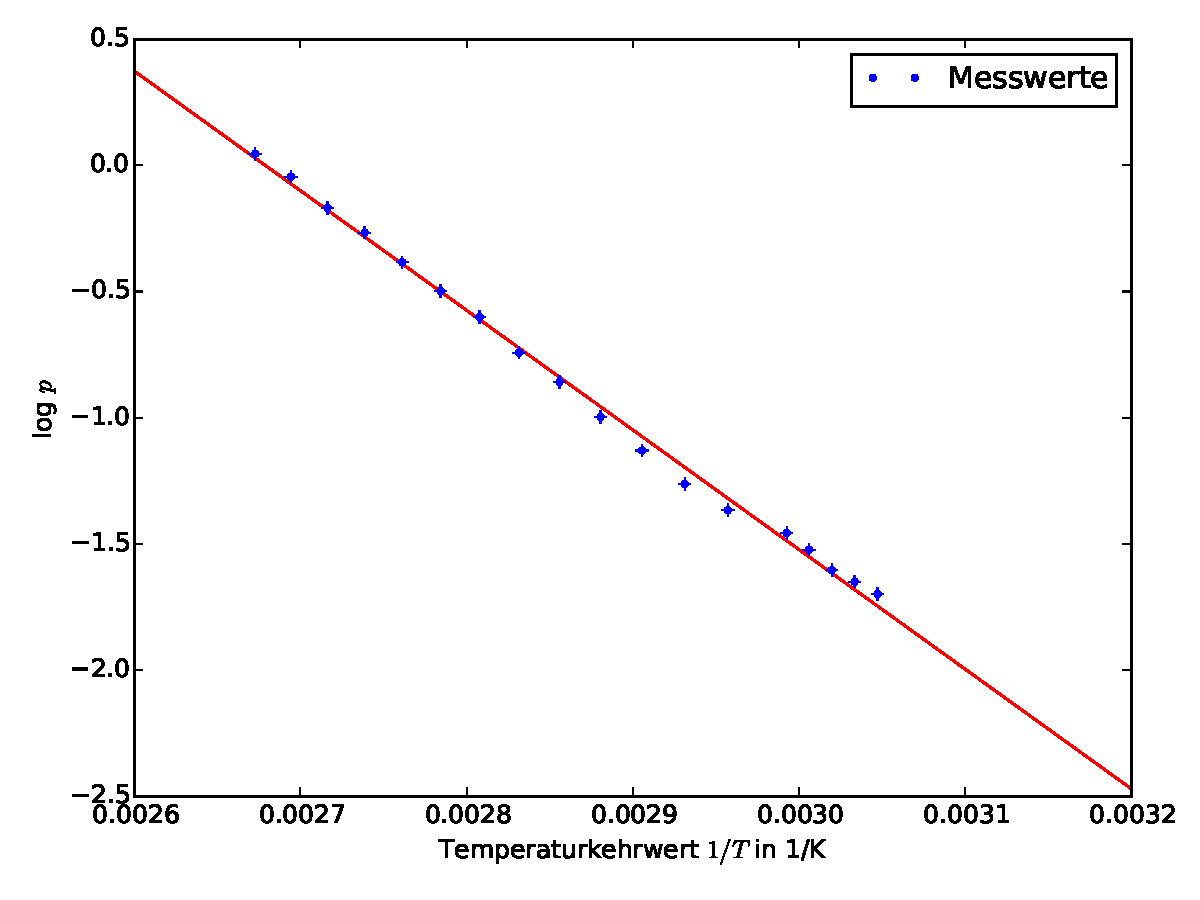
\includegraphics[width=0.78\textwidth]{verdampfungwaerme1.pdf}
  \caption{Fit und Messwerte im Niedrigdruckbereich.}
  \label{fig:fit1}
\end{figure}
In Tabelle \ref{tab:messung2} sind die gemessenden Wertetupel für die Messreihe
$p>1\si{\bar}$ angegeben. In Abbildung \ref{fig:fit2} wird der Dampfdruck in Abhängigkeit
von der Temperatur aufgetragen. Die Temperaturabhängige Verdampfungswärme
ergibt sich bei Vernachlässigung von $V_F$, durch die Umformungen
\begin{align}
  RT=&\left(p+\frac{a}{V_D^2}V_D\right)\\
  V_D=&\frac{RT}{2p}\sqrt{\frac{R^2T^2}{4p^2}-\frac{a}{p}}\;\;,
\end{align}
und dem einsetzen in Gleichung \eqref{eqn:clausius_vereinfacht} durch
\begin{align}
  L=&\frac{T}{p}\left[\frac{RT}{2p}\pm\sqrt{\frac{R^2T^2}{4p^2}-\frac{a}{p}}\right]\frac{\text{d}p}{\text{d}T}\;\;.
\end{align}
Die Konstante ist $a=0.9\si{\frac{\joule\meter^3}{\mol^2}}$ . Um den Differentialquotienten $\frac{\text{d}p}{\text{d}T}$ zu berchnen wird
mit den Wertepaaren aus Tabelle \ref{tab:messung2} ein Ausgleichspolynom 3.Grades
erstellt. Der Fit hat die Form
\begin{equation}
  p(T)=AT^3+B T^2+CT+D
\end{equation}
mit den Fitparametern
\begin{align*}
  A=&\SI{-6(3)e-1}{\frac{\pascal}{\kelvin}}\\
  B=&\SI{ 8(3)e2}{\frac{\pascal}{\kelvin}}\\
  C=&\SI{-3(1)e5 }{\frac{\pascal}{\kelvin}}\\
  D=&\SI{ 5(2)e7 }{\pascal}\;\;.
\end{align*}
Der Differentialquotient $\frac{\text{d}p}{\text{d}T}$ hat damit die Form
\begin{equation*}
  3AT^2+2BT+C\;\;.
\end{equation*}
Die Temperaturabhängige Verdampfungswärme ist demnach
\begin{equation*}
  L(T)=\left[\frac{RT}{2}\pm\sqrt{\left(\frac{RT}{2}\right)^2-a(AT^3+BT^2+CT+D)}\right]
  \frac{3AT^3+2BT^2+CT}{AT^3+BT^2+CT+D}\;\;.
  \label{eqn:Verdampfungswaerme_t}
\end{equation*}

\begin{table}
  \centering
  \begin{tabular}{c c c }
    \toprule
    Temperatur & Druck gemessen & Druck ohne Offset\\
    $T$ in $\si{\kelvin}$ & $p_m$ in $ 10^2\si{\bar}$ &$p$ in $ 10^2\si{\bar}$ \\
    \midrule
    373.15  &  -5.74  &  1.00  \\
    374.15  &  -5.68  &  1.06  \\
    375.15  &  -5.66  &  1.08  \\
    376.15  &  -5.61  &  1.13  \\
    377.15  &  -5.57  &  1.17  \\
    378.15  &  -5.52  &  1.22  \\
    379.15  &  -5.47  &  1.27  \\
    380.15  &  -5.42  &  1.32  \\
    381.15  &  -5.37  &  1.37  \\
    382.15  &  -5.31  &  1.43  \\
    383.15  &  -5.25  &  1.49  \\
    384.15  &  -5.20  &  1.54  \\
    385.15  &  -5.14  &  1.60  \\
    386.15  &  -5.08  &  1.66  \\
    387.15  &  -5.01  &  1.73  \\
    388.15  &  -4.95  &  1.79  \\
    389.15  &  -4.88  &  1.86  \\
    390.15  &  -4.81  &  1.93  \\
    391.15  &  -4.75  &  1.99  \\
    392.15  &  -4.68  &  2.06  \\
    393.15  &  -4.60  &  2.14  \\
    394.15  &  -4.52  &  2.22  \\
    395.15  &  -4.46  &  2.28  \\
    396.15  &  -4.38  &  2.36  \\
    397.15  &  -4.30  &  2.44  \\
    398.15  &  -4.22  &  2.52  \\
    399.15  &  -4.14  &  2.60  \\
    \bottomrule
  \end{tabular}
  \caption{}
  \label{tab:messung2}
\end{table}
\begin{figure}
  \centering
  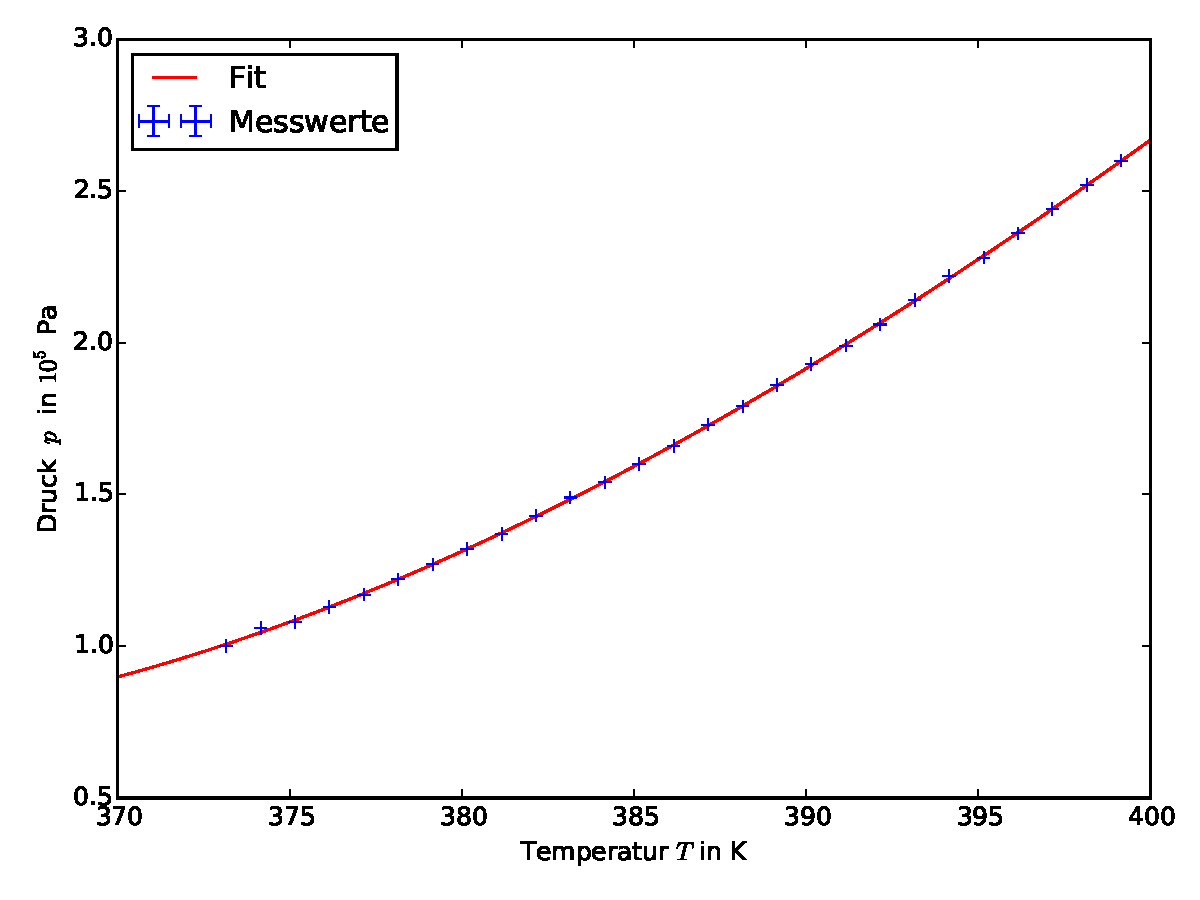
\includegraphics[width=0.78\textwidth]{verdampfungwaerme2.pdf}
  \caption{Ausgleichspolynom und Messwerte im Hochdruckbereich..}
  \label{fig:fit2}
\end{figure}
Setzt man in Gleichung \eqref{eqn:Verdampfungswaerme_t} die Gemessenden Temperaturwerte ein erhält man
die temperaturabhängige Verdampfungswärme, die in den Abbildungen \ref{fig:fit3} und \ref{fig:fit4}
dargestellt ist.
\begin{figure}
  \centering
  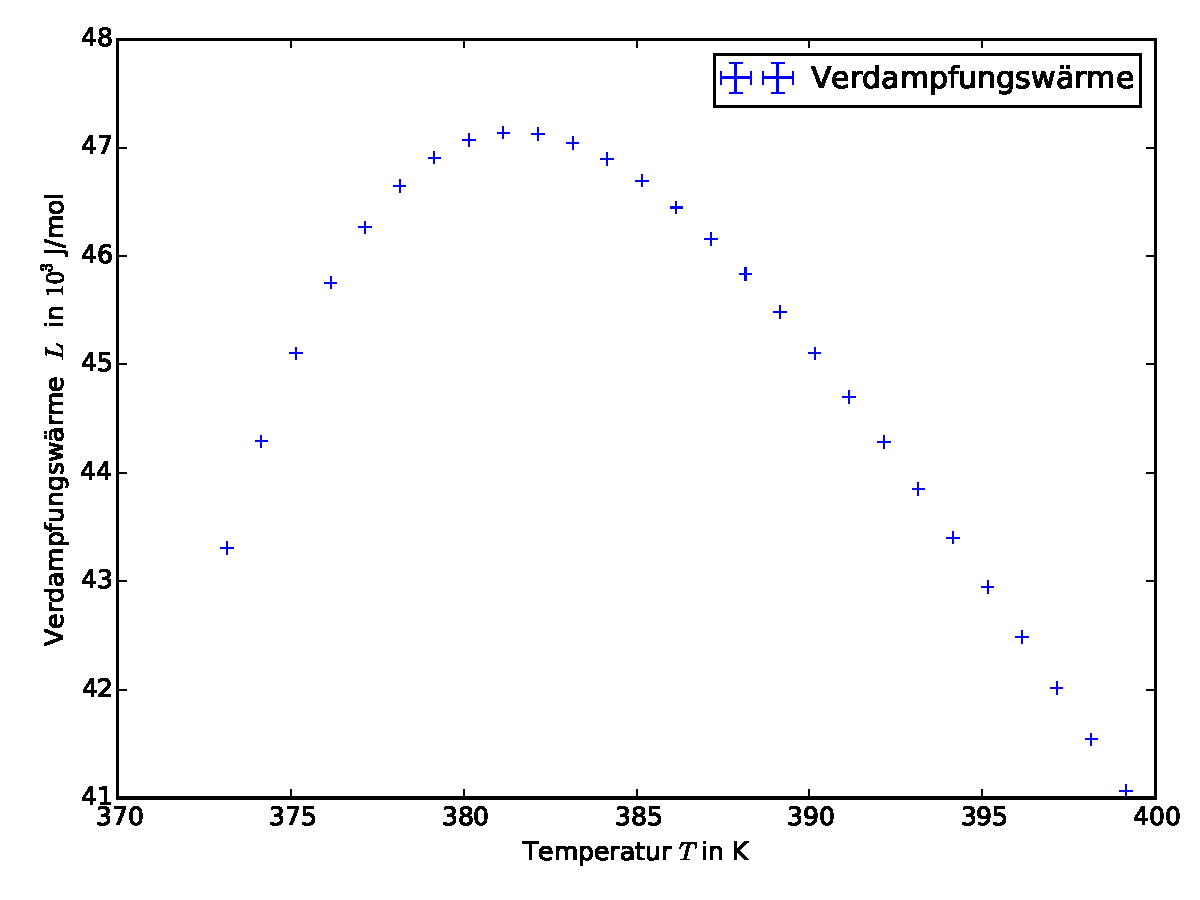
\includegraphics[width=0.82\textwidth]{verdampfungwaerme3.pdf}
  \caption{Temperaturabhängige Verdampfungswärme bei positiver Wurzel.}
  \label{fig:fit3}
\end{figure}
\begin{figure}
  \centering
  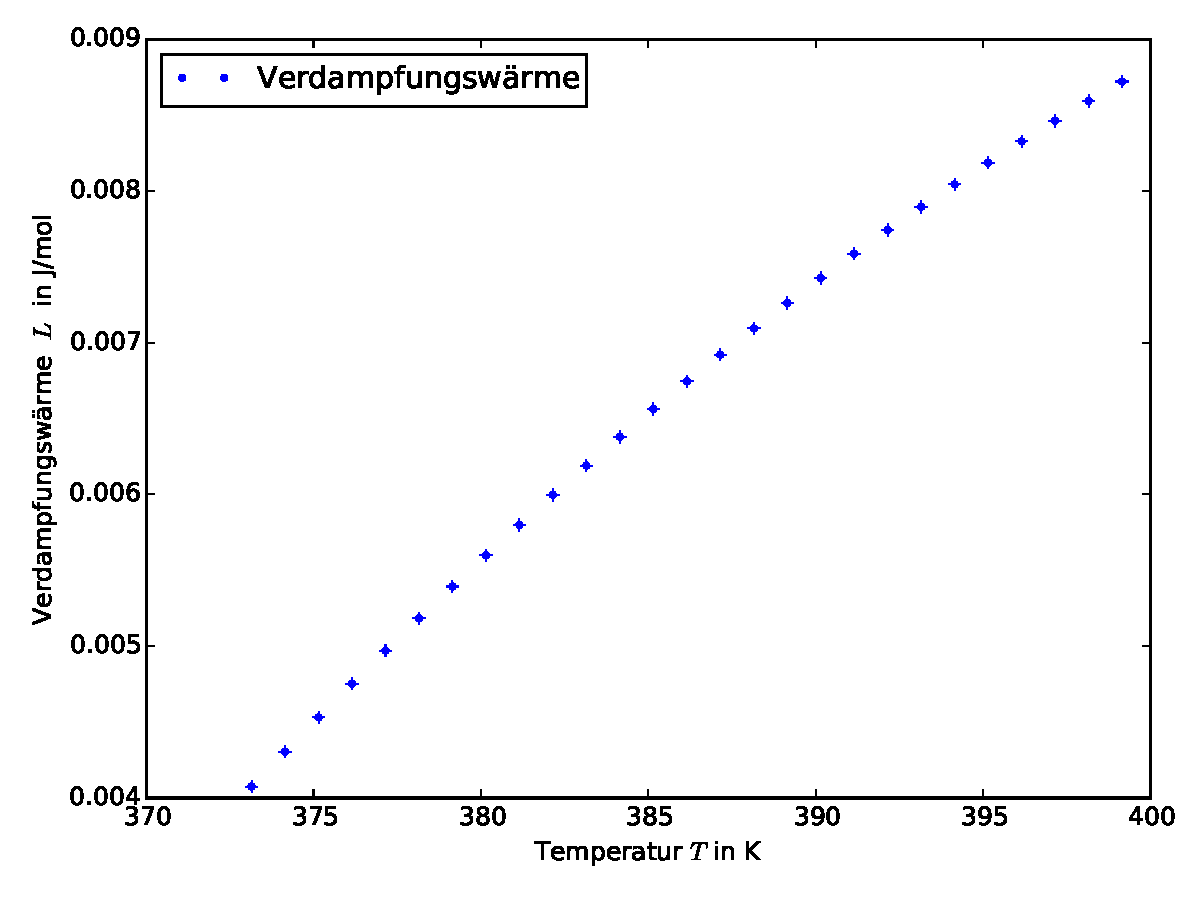
\includegraphics[width=0.78\textwidth]{verdampfungwaerme4.pdf}
  \caption{Temperaturabhängige Verdampfungswärme bei negativer Wurzel.}
  \label{fig:fit4}
\end{figure}
